\documentclass[bachelor, och, labwork]{shiza}
% параметр - тип обучения - одно из значений:
%    spec     - специальность
%    bachelor - бакалавриат (по умолчанию)
%    master   - магистратура
% параметр - форма обучения - одно из значений:
%    och   - очное (по умолчанию)
%    zaoch - заочное
% параметр - тип работы - одно из значений:
%    referat    - реферат
%    coursework - курсовая работа (по умолчанию)
%    diploma    - дипломная работа
%    pract      - отчет по практике
% параметр - включение шрифта
%    times    - включение шрифта Times New Roman (если установлен)
%               по умолчанию выключен
\usepackage{subfigure}
\usepackage{tikz,pgfplots}
\pgfplotsset{compat=1.5}
\usepackage{float}

%\usepackage{titlesec}
\setcounter{secnumdepth}{4}
%\titleformat{\paragraph}
%{\normalfont\normalsize}{\theparagraph}{1em}{}
%\titlespacing*{\paragraph}
%{35.5pt}{3.25ex plus 1ex minus .2ex}{1.5ex plus .2ex}

\titleformat{\paragraph}[block]
{\hspace{1.25cm}\normalfont}
{\theparagraph}{1ex}{}
\titlespacing{\paragraph}
{0cm}{2ex plus 1ex minus .2ex}{.4ex plus.2ex}

% --------------------------------------------------------------------------%


\usepackage[T2A]{fontenc}
\usepackage[utf8]{inputenc}
\usepackage{graphicx}
\graphicspath{ {./images/} }
\usepackage{tempora}

\usepackage[sort,compress]{cite}
\usepackage{amsmath}
\usepackage{amssymb}
\usepackage{amsthm}
\usepackage{fancyvrb}
\usepackage{listings}
\usepackage{listingsutf8}
\usepackage{longtable}
\usepackage{array}
\usepackage[english,russian]{babel}

\usepackage[colorlinks=false]{hyperref}
\usepackage{url}

\usepackage{underscore}
\usepackage{setspace}
\usepackage{indentfirst} 
\usepackage{mathtools}
\usepackage{amsfonts}
\usepackage{enumitem}
\usepackage{tikz}
\usepackage{minted}

\newcommand{\eqdef}{\stackrel {\rm def}{=}}
\newcommand{\specialcell}[2][c]{%
\begin{tabular}[#1]{@{}c@{}}#2\end{tabular}}

\renewcommand\theFancyVerbLine{\small\arabic{FancyVerbLine}}

\newtheorem{lem}{Лемма}

\begin{document}

% Кафедра (в родительном падеже)
\chair{теоретических основ компьютерной безопасности и криптографии}

% Тема работы
\title{Универсальные алгебры и алгебра отношений}

% Курс
\course{3}

% Группа
\group{331}

% Факультет (в родительном падеже) (по умолчанию "факультета КНиИТ")
\department{факультета КНиИТ}

% Специальность/направление код - наименование
%\napravlenie{09.03.04 "--- Программная инженерия}
%\napravlenie{010500 "--- Математическое обеспечение и администрирование информационных систем}
%\napravlenie{230100 "--- Информатика и вычислительная техника}
%\napravlenie{231000 "--- Программная инженерия}
\napravlenie{10.05.01 "--- Компьютерная безопасность}

% Для студентки. Для работы студента следующая команда не нужна.
% \studenttitle{Студентки}

% Фамилия, имя, отчество в родительном падеже
\author{Токарева Никиты Сергеевича}

% Заведующий кафедрой
% \chtitle{} % степень, звание
% \chname{}

%Научный руководитель (для реферата преподаватель проверяющий работу)
\satitle{аспирант} %должность, степень, звание
\saname{В. Н. Кутин}

% Руководитель практики от организации (только для практики,
% для остальных типов работ не используется)
% \patitle{к.ф.-м.н.}
% \paname{С.~В.~Миронов}

% Семестр (только для практики, для остальных
% типов работ не используется)
%\term{8}

% Наименование практики (только для практики, для остальных
% типов работ не используется)
%\practtype{преддипломная}

% Продолжительность практики (количество недель) (только для практики,
% для остальных типов работ не используется)
%\duration{4}

% Даты начала и окончания практики (только для практики, для остальных
% типов работ не используется)
%\practStart{30.04.2019}
%\practFinish{27.05.2019}

% Год выполнения отчета
\date{2022}

\maketitle

% Включение нумерации рисунков, формул и таблиц по разделам
% (по умолчанию - нумерация сквозная)
% (допускается оба вида нумерации)
% \secNumbering

%-------------------------------------------------------------------------------------------

\section{Постановка задачи}

    \textbf{Цель работы} -- изучение основных понятий универсальной алгебры и операций над бинарными отношениями. 

    Порядок выполнения работы:
    \begin{enumerate}
        \item Рассмотреть понятие алгебраической операции и классификацию свойств операций. Разработать
        алгоритмы проверки свойств операций: ассоциативность, коммутативность, идемпотентность, обратимость, дистрибутивность.
        \item Рассмотреть основные операции над бинарными отношениями. Разработать алгоритмы выполнения
        операции над бинарными отношениями.
        \item Рассмотреть основные операции над матрицами. Разработать алгоритмы выполнения операций над матрицами.
    \end{enumerate}

\section{Теоретические сведения по рассмотренным темам с их обоснованием}

    \subsection{Понятие алгебраической операции}

    Отображение $f : A^n \rightarrow A$ называется алгебраической $n$-арной операцией или просто 
    \textbf{алгебраической операцией} на множестве $A$. При этом $n$ называется порядком или арностью алгебраической операции $f$.
    
    Далее для бинарной операции $f$ по возможности будем использовать мультипликативную запись с помощью символа <<$\cdot$>>,
    т.е.вместо $f(x,y)$ писать $x \cdot y$. При необходимости для бинарной операции $f$ используется также аддитивная запись
    с помощью символа <<$ + $>>, т.е. вместо $f(x,y)$ записывается $x + y$.

    
    \subsection{Классификация свойств операций}

    Бинарная операция $\cdot$ на множестве A называется:

    \begin{itemize}
        \item идемпотентной, если $\forall x \in A$ выполняется равенство $x \cdot x = x$;

        \item коммутативной, если $\forall x, y \in A$ выполняется равенство $x \cdot y = y \cdot x$;

        \item ассоциативной, если $\forall x, y, z \in A$ выполняется равенство $x \cdot (y \cdot z) = (x \cdot y) \cdot z$;

        \item обратимой, если $\forall x, y \in A$, если уравнения $x \cdot a = y$ и $b \cdot x = y$  имеют решение, причем единственное;
        \item дистрибутивной относительно операции +, если $\forall x, y, z \in A$ выполняются равенства
        
        \begin{center}
            $x \cdot (y + z) = (x \cdot y) + (x \cdot z)$,

            $(y + z) \cdot x = (y \cdot x) + (z \cdot x)$;
        \end{center}
    \end{itemize}

    \subsection{Основные операции над бинарными отношениями}

    \begin{itemize}
        \item Над бинарными отношениями можно выполнять любые теоретико-множественные операции, в частности операции
        объединения $\cup$ и пересечения $\cap$;
        \item Обратным для бинарного отношения $\rho \subset A \times B$ называется бинарное
        отношение $\rho^{-1} \subset B \times A$, определяющееся по формуле:
        \begin{center}
            $\rho^{-1} = \{(b, a) : (a, b) \in \rho \}$;
        \end{center}
        \item Композицией бинарных отношений $\rho \subset A \times B$ и $\sigma \subset B \times C$
        называется бинарное отношение $\rho \circ \sigma \subset A \times C$, определяющееся по формуле:
        \begin{center}
            $\rho \circ \sigma = \{ (a, c) : (a, b) \in \rho \text{ и } (b, c) \in \sigma \text{ для некоторого } b \in B \}$;
        \end{center}
    \end{itemize}

    \subsection{Основные операции над матрицами}

    \begin{itemize}
            \item Сложение и вычитание матриц.
        
            Суммой $A + B$ матриц $A_{m \times n} = (a_{ij}) \text{ и }B_{m \times n} = (b_{ij})$ называется матрица 
            $C_{m \times n} = (c_{ij})$ , где $c_{ij} = a_{ij} + b_{ij}$ для всех $i = \overline{1, m} \text{ и } j = \overline{1, n}$ .

            Разностью $A - B$ матриц $A_{m \times n} = (a_{ij}) \text{ и }B_{m \times n} = (b_{ij})$ называется матрица 
            $C_{m \times n} = (c_{ij})$ , где $c_{ij} = a_{ij} - b_{ij}$ для всех $i = \overline{1, m} \text{ и } j = \overline{1, n}$ .

        \item Умножение матрицы на число.
        
            Произведением матрицы $A_{m \times n} = (a_{ij}) \text{ на число } \alpha$ называется матрица 
            $C_{m \times n} = (c_{ij})$ , где $c_{ij} = \alpha a_{ij}$ для всех $i = \overline{1, m} \text{ и } j = \overline{1, n}$ .

        \item Произведение двух матриц.
        
            Произведением матриц $A_{m \times n} = (a_{ij}) \text{ на матрицу }B_{m \times n} = (b_{ij})$ называется матрица 
            $C_{m \times n} = (c_{ij})$ , где $c_{ij} = \sum\limits_{k=1}^n a_{ik}b_{kj}$ для всех $i = \overline{1, m} \text{ и } j = \overline{1, n}$.
        
        \item Транспонирование матрицы.
        
            Транспонированной по отношению к матрице $A_{m \times n} = (a_{ij})$ называется матрица $A^T_{n \times m} = (a^T_{ij})$
            для элементов которой $a^T_{ij} = a_{ji}$.
        
        \item Обращение матрицы.

            Обращение матрицы $A_{m \times n}$ - получение матрицы $A^{-1}$, обратной к исходной матрице $A$. Обратная
            матрица $A^{-1}$ "--- такая, при умножении которой на исходную матрицу $A$ получается единичная матрица $E$.
            Это такая матрица, которая удовлетворяет равенству \[AA^{-1} = A^{-1}A = E\] 

    \end{itemize}


    % В решеточно упорядоченном множестве $A = (A, \leq)$ определены две бинарные операции $a \wedge b = inf\{a, b\}$ и $a \vee b = sup\{a, b\}$.
    % Операция $\wedge$ называется \textbf{пересечением} и операция $\vee$ -- \textbf{объединением}. Эти операции решетки взаимосвязаны с ее порядком
    % по формулам:
    % \begin{center}
    %     $a \leq b \iff a \wedge b = a$ и $a \leq b \iff a \vee b = b$.
    % \end{center}

    % Свойства операций решетки:

    % \begin{enumerate}
    %     \item $a \wedge a = a$, $a \vee a = a$ -- идемпотентность операций $\wedge$, $\vee$;
    %     \item $a \wedge b = b \wedge a$, $a \vee b = b \vee a$ -- коммутативность операций $\wedge$, $\vee$;
    %     \item $(a \wedge b) \wedge c = a \wedge (b \wedge c)$, $(a \vee b) \vee c = a \vee (b \vee c)$ -- ассоциативность операций $\wedge$, $\vee$;
    %     \item $a \wedge (a \vee b) = a$, $a \vee (a \wedge b) = a$ -- законы поглощения;
    %     \item Решетка $A$ называется дистрибутивной, если $\forall a$, $b$, $c \in A$ выполняются равенства:
        
    %     \begin{center}
    %         $(a \wedge b) \vee c = (a \vee c) \wedge (b \vee c)$, 
            
    %         $(a \vee b) \wedge c = (a \wedge c) \vee (b \wedge c)$.
    %     \end{center}
    % \end{enumerate}




\section{Результаты работы}
    
    \subsection{Коды программ, реализующей рассмотренные алгоритмы}


        \inputminted[fontsize=\small]{Python}{code/aua-lab3.py}








    \subsection{Результаты тестирования программ}
    
        % \begin{figure}[H]
        %     \centering
        %     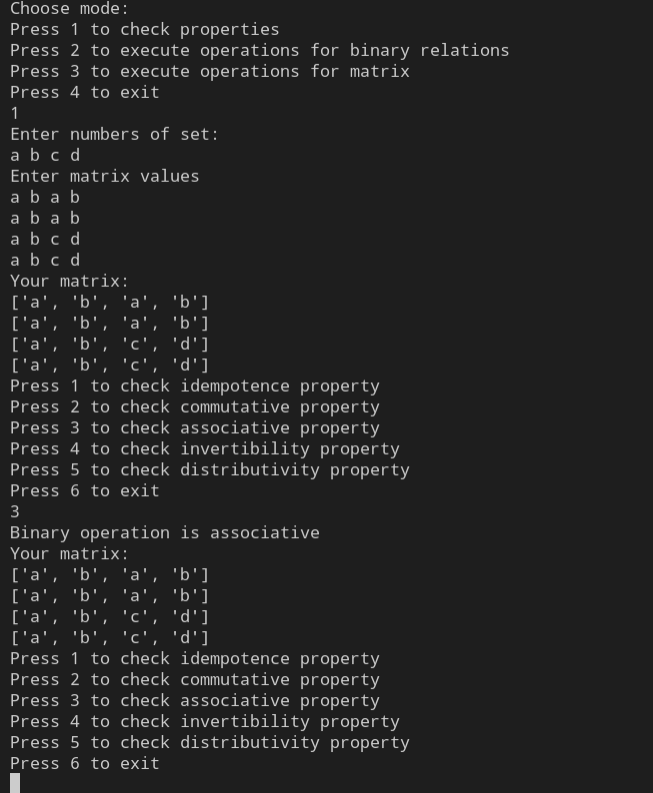
\includegraphics[width=0.8\textwidth]{photo/1.png}
        %     \caption{Тест алгоритма построения эквивалентного замыкания}
        % \end{figure}

        % \begin{figure}[H]
        %     \centering
        %     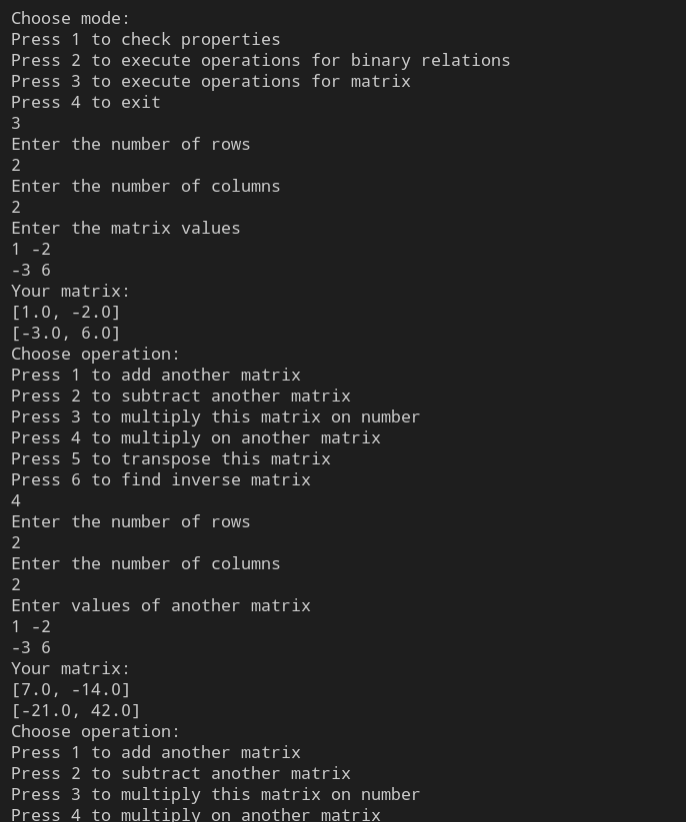
\includegraphics[width=1\textwidth]{photo/2.png}
        %     \caption{Тест алгоритма построения диаграммы Хассе на множестве ($X$, $|$)}
        % \end{figure}

        % \begin{figure}[H]
        %     \centering
        %     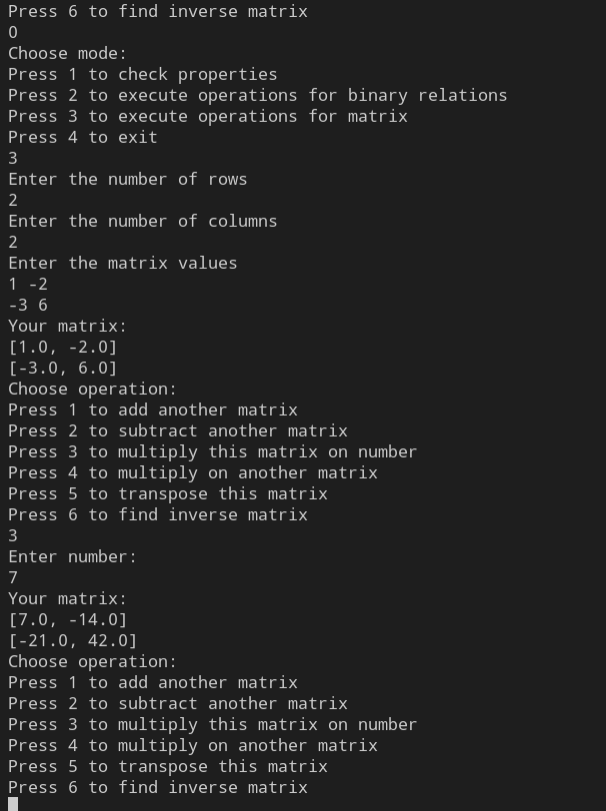
\includegraphics[width=1\textwidth]{photo/3.png}
        %     \caption{Тест алгоритма построения диаграммы Хассе на множестве ($X$, $\leq$)}
        % \end{figure}

        % \begin{figure}[H]
        %     \centering
        %     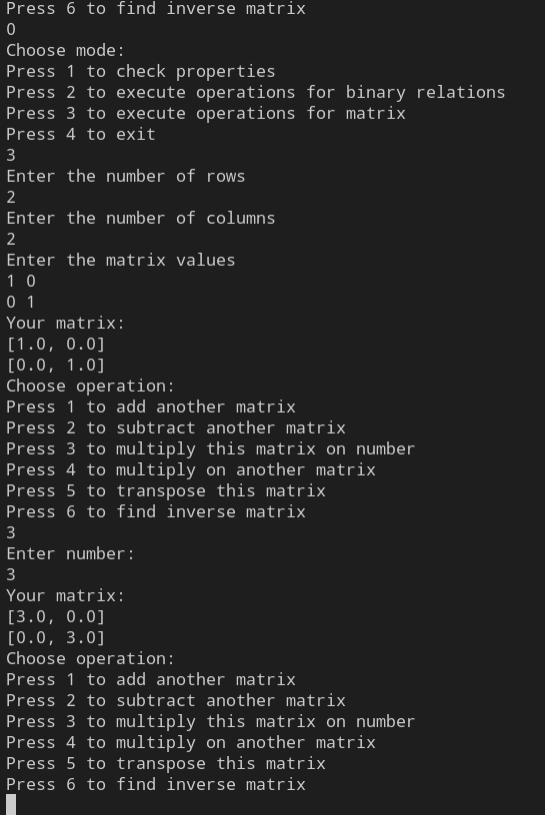
\includegraphics[width=1\textwidth]{photo/4.png}
        %     \caption{Тест алгоритма построения решетки концептов}
        % \end{figure} 
    \newpage
 
    \conclusion
    
    В результате лабораторной работы были рассмотрены теоретические сведения об отношении эквивалентности, разобраны
    определения фактор-множества, отношения порядка и диаграммы Хассе, контекста и концепта. Опираясь на изложенную
    выше теорию, были разработаны алгоритмы построения эквивалентного замыкания бинарного отношения и системы представителей
    фактор-множества, алгоритмы вычисления минимальных (максимальных) и наименьших (наибольших) элементов и построения
    диаграммы Хассе, а также алгоритмы построения решетки концептов. Была произведена оценка сложности каждого из 
    построенных алгоритмов. Была реализована программа, написанная на языке Python.
    
\end{document}